\documentclass{beamer}
\usepackage{beamerthemesplit}
\usepackage {graphicx}
\usepackage{psfrag}
\useoutertheme{shadow}
\useoutertheme{split}
\usepackage{color}
%\usetheme{Madrid}
\usetheme{Warsaw}

\usepackage{listings}

\lstset{language=Python,
    basicstyle=\ttfamily\bfseries,
    commentstyle=\color{red}\itshape,
  stringstyle=\color{darkgreen},
  showstringspaces=false,
  keywordstyle=\color{blue}\bfseries}

\newtheorem{assumption}{Assumption}
%\newtheorem{definition}{Definition}
\newtheorem {proposition} {Proposition}
\newtheorem {propos} {Proposition}
\newtheorem{thm}{Theorem}
\newtheorem{result}{Result}
\newtheorem{formula}{Formula}
\usepackage[font={small,it}]{caption}


\date{December 18, 2018}
\title[Machine Learning 2018 -- Dimensionality Reduction]
{ Machine Learning 2018 --  Dimension Reduction \\
}

\titlegraphic{
 	  \centering

\includegraphics[scale=0.1]{VEF_logo_FN.png} }

%\subtitle{A package for use with prosper}
\author [Trung Le] {Trung Le}

\begin{document}
\frame{\titlepage}

\frame{
\frametitle{Dimensionality Reduction}
How to visualize this dataset ?
\begin{table}[]
	\begin{tabular}{|l|l|l|l|l|}
		\hline
		Sepal length & Sepal width & Petal length & Petal width & Class     \\ \hline
		5.1 & 3.5 & 1.4 & 0.2 & Setosa     \\ \hline
		4.9 & 3.0 & 1.4 & 0.2 & Setosa     \\ \hline
		7.0 & 3.2 & 4.7 & 1.4 & Versicolor \\ \hline
		6.4 & 3.2 & 4.5 & 1.5 & Versicolor \\ \hline
		6.3 & 2.9 & 5.6 & 1.8 & Virginica  \\ \hline
		5.9 & 3.0 & 5.1 & 1.8 & Virginica  \\ \hline
	\end{tabular}
\end{table}
}

\frame{
\frametitle{Dimensionality Reduction}
\centering
\begin{figure}
	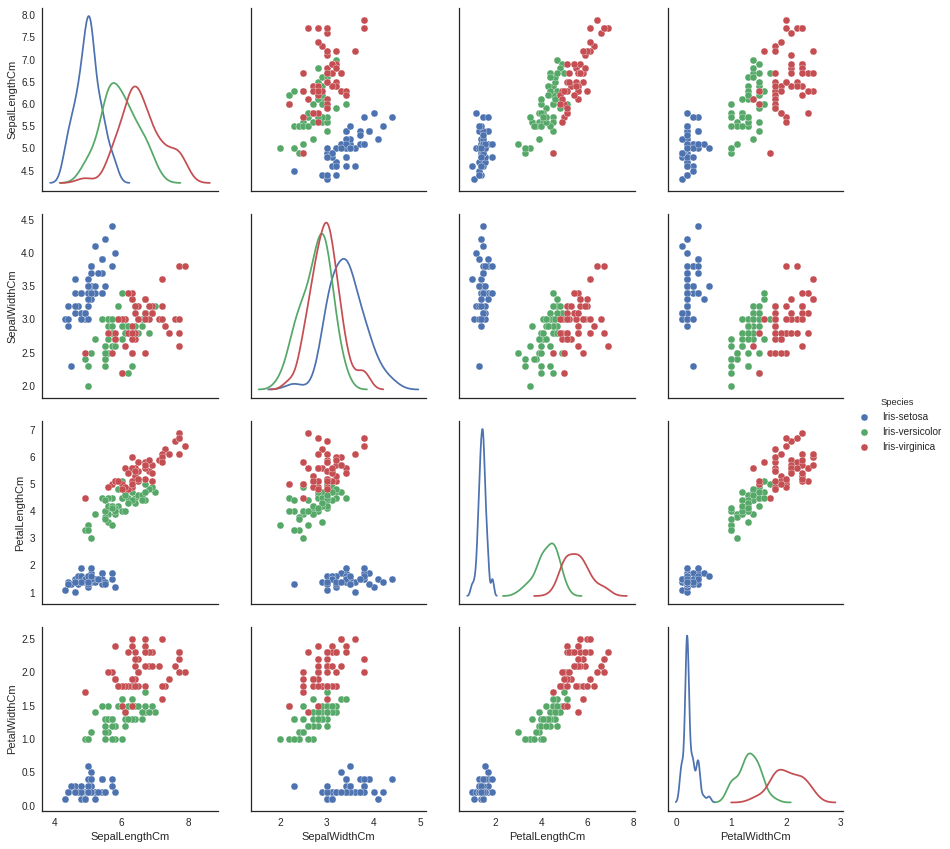
\includegraphics[scale=0.2]{iris-pairplot.png}
	\caption{Pair plot of iris dataset, source: kaggle.com}
\end{figure}
}

\frame{
	\frametitle{Dimensionality Reduction}
	\begin{itemize}
	\item The number of such plots required for such visualizing data of $n$ variables is $O(n^2)$
	\item The simplest way to reduce the dimension is by taking a random projection of the data.
	\item Though random projection allows some degree of visualization of the data structure, it is likely that the more interesting structure within the data will be lost.
	\end{itemize}
}

\frame{
	\frametitle{Dimensionality Reduction}
	\begin{itemize}
	\item Dimensionality Reduction tries to express the data in lower dimension without losing too much information. \\
	\item Why dimensionality reduction ?
	\begin{itemize}
	    \item Reduce the dimensions of data to 2D or 3D to visualize it precisely.
		\item Help in data compressing and reducing the storage space.
		\item Remove redundant features, if any.
	\end{itemize}
	\item Some of dimension reduction methods: PCA, t-SNE, LDA,...
	\end{itemize}
}

\frame{
\frametitle{Dimensionality Reduction}
\centering
\begin{figure}
	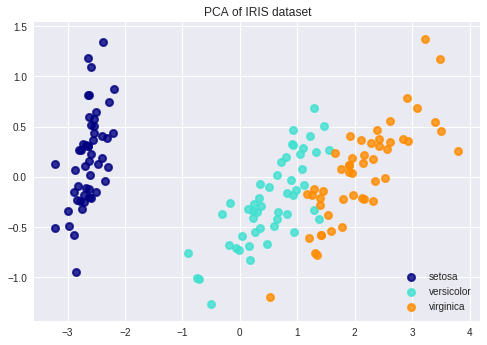
\includegraphics[scale=0.5]{iris-pca.png}
	\caption{PCA of IRIS dataset, source: scikit-learn.org}
\end{figure}
}

\frame{
\frametitle{Background Mathematics}
Given a dataset $X \in \mathbb{R}^{N \times D}$
\begin{itemize}
	\item Mean: $\bar{X_i} = \frac{1}{N}\sum_{j=1}^{N}X_{ij}$
	\item Variance: $Var(X_i) = \frac{1}{N}\sum_{j=1}^{N}(X_{ij}-\bar{X_i})^2$
	\item Covariance: $Cov(X_i, X_k) = Cov(X_k, X_i) =  \frac{1}{N}\sum_{j=1}^{N}(X_{ij}-\bar{X_i})(X_{kj}-\bar{X_k})$
\end{itemize}
}

\frame{
\frametitle{Covariance}
\begin{figure}[!htb]
	\minipage{0.4\textwidth}
	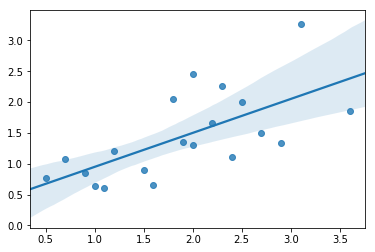
\includegraphics[width=\linewidth]{positive-cov.png}
	%\caption{Positive covariance}
	\endminipage\hfill
	\minipage{0.4\textwidth}
	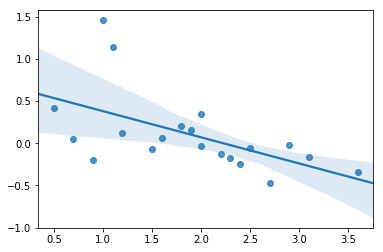
\includegraphics[width=\linewidth]{negative-cov.png}
	%\caption{Negative covariance}
	\endminipage\hfill
	\minipage{0.4\textwidth}%
	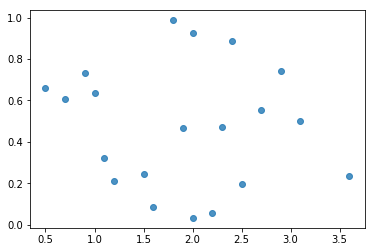
\includegraphics[width=\linewidth]{no-cov.png}
	%\caption{Zero covariance}
	\endminipage
	\caption{Positive, negative and zero covariance}
\end{figure}
}

\frame{
\frametitle{Covariance Matrix}
\begin{itemize}
    \item Covariance matrix of $X \in \mathbb{R}^{N \times D}$
\begin{equation}
\Sigma = 
\begin{pmatrix}
    Var(X_1) & Cov(X_1,X_2) & \ldots & Cov(X_1,X_D) \\
    Cov(X_2,X_1) & Var(X_2) & \ldots & Cov(X_1,X_D) \\
    \vdots & \vdots & \vdots & \ldots \\
    Cov(X_D,X_1) & Cov(X_D,X_2) & \ldots & Var(X_D)
\end{pmatrix}
\end{equation}
    \item For centered data:
$\Sigma = \frac{1}{N}XX^T$
where $X$ is re-constructed by subtracting every column by it's mean $X_i = X_i - \bar{X_i}$.
\end{itemize}
}

\frame{
\frametitle{Principal Component Analysis (PCA)}
\centering
\begin{figure}
	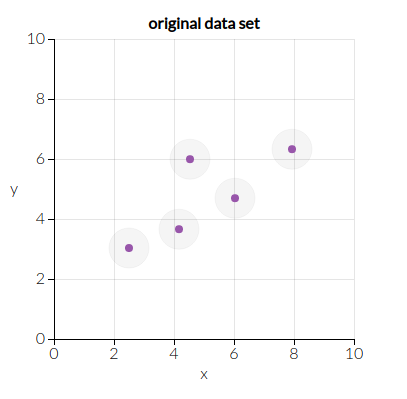
\includegraphics[scale=0.5]{ori.png}
	\caption{Sample data points in 2D}
\end{figure}
}

\frame{
\frametitle{Principal Component Analysis (PCA)}
\centering
\begin{figure}
	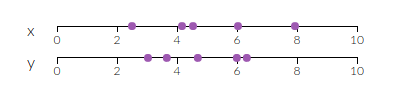
\includegraphics[scale=0.5]{ori-data-variance.png}
	\caption{Sample data points in 2D}
\end{figure}
}

\frame{
\frametitle{Principal Component Analysis (PCA)}
\centering
\begin{figure}
	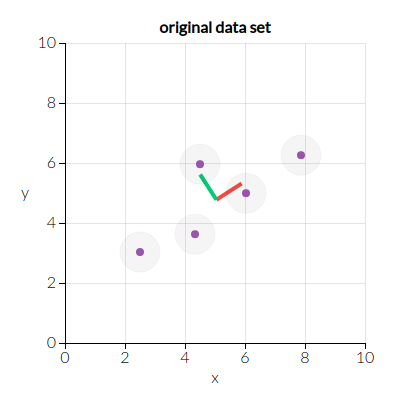
\includegraphics[scale=0.5]{pca-on-original-axis.png}
	\caption{PCA of sample data points in 2D}
\end{figure}
}

\frame{
\frametitle{Principal Component Analysis (PCA)}
\centering
\begin{figure}
	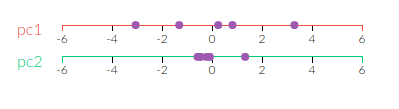
\includegraphics[scale=0.5]{pca-variance.png}
	\caption{PCA of sample data points in 2D}
\end{figure}
}

\frame{
\frametitle{Principal Component Analysis (PCA)}
\begin{itemize}
    \item Algebraically, principal components are particular linear combinations of the $D$ random variables $X_1, X_2, ..., X_D$.
    \item Geometrically, these linear combinations represent the selection of a new coordinate system obtained by rotating the original system.
\end{itemize}
}

\frame{
\frametitle{Principal Component Analysis (PCA)}
\begin{itemize}
    \item Let $X \in \mathbb{R}^{N \times D}$ is the original data matrix with $N$ samples and $D$ measurements.
    % \item $X$ has the covariance matrix $\Sigma$ with eigenvalues $\lambda_1 \ge \lambda_2 \ge..\ge \lambda_D \ge 0$.
    \item Consider the linear combinations:
    \begin{equation}
    \begin{align}
            Y_1 &= w_1^TX &= w_{11}X_1 + w_{12}X_2 + ... + w_{1D}X_D \\
            Y_2 &= w_2^TX &= w_{21}X_1 + w_{22}X_2 + ... + w_{2D}X_D \\
            \vdots \\
            Y_D &= w_D^TX &= w_{D1}X_1 + w_{D2}X_2 + ... + w_{DD}X_D
    \end{align}
    \end{equation}
    where $w \in \mathbb{R}^{D \times D}$
\end{itemize}
}

\frame{
\frametitle{Principal Component Analysis (PCA)}
    \centering
    \begin{figure}
    	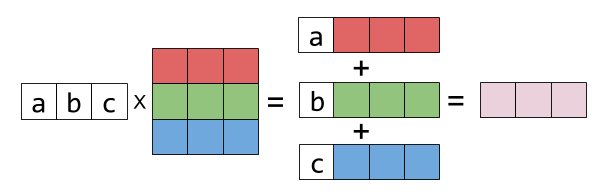
\includegraphics[scale=0.5]{matrixmul.png}
    	\caption{Matrix multiplication visualization, source: eli.thegreenplace.net}
    \end{figure}
}

\frame{
\frametitle{Principal Component Analysis (PCA)}
    \centering
    \begin{figure}
    	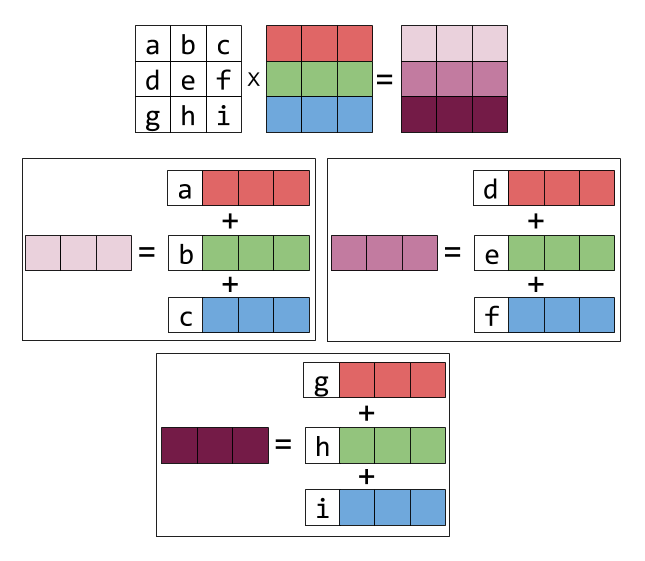
\includegraphics[scale=0.4]{matrixmulmatrix.png}
    	\caption{Matrix multiplication visuallization, source: eli.thegreenplace.net}
    \end{figure}
}

\frame{
\frametitle{Principal Component Analysis (PCA)}
The important point to note is that the variance of any linear combination can be computed using the covariance matrix of the data:
\begin{equation}
\begin{align}
    Var(Y_i) &= \frac{1}{N} \sum_j (X_j w_i)^2 \\
             &= \frac{1}{N} (X w_i)^T (X w_i) \\
             &= \frac{1}{N} w_i^T X^T X w_i \\
             &= w_i^T \frac{X^T X}{N} w_i \\
             &= w_i^T \Sigma w_i
\end{align}
\end{equation}
}

\frame{
\frametitle{Principal Component Analysis (PCA)}
\begin{itemize}
    \item Principal components are those linear combinations $Y_1, Y_2,...,Y_D$ whose variances are as large as possible.
    \item First principal component: Linear combination $w_1^TX$ that maximize $Var(w_1^TX)$ subject to $||w_1||_2^2 = 1$
    \item Second principal component: Linear combination $w_2^TX$ that maximize $Var(w_2^TX)$ subject to $||w_2||_2^2 = 1$ and $w_2^Tw_1 = 0$
    \item $i$th principal component: Linear combination $w_i^TX$ that maximize $Var(w_i^TX)$ subject to $||w_i||_2^2 = 1$ and $w_i^Tw_k = 0$ for $k < i$
\end{itemize}
}

\frame{
\frametitle{First Principal Component Analysis (PC1)}
    For the first principal component, we maximize:
    \begin{equation}
        Var(Y_1) = w_1^T \Sigma w_1
    \end{equation} subject to: 
    \begin{equation}
        w_1^Tw_1 = 1
    \end{equation}
}

\frame{
\frametitle{First Principal Component Analysis (PC1)}
    Using the Lagrange function:
    \begin{equation}
        \mathcal{L} = w_1^T \Sigma w_1 + \lambda_1 (1 - w_1^T w_1)
    \end{equation}
    Taking the partial derivative of $\mathcal{L}$ with respect to $w_1$, $\lambda_1$:
    \begin{equation}
        \label{partialw}
        \frac{\partial}{\partial w_1}\mathcal{L}(w_1, \lambda_1) = 2\Sigma w_1 - 2\lambda_1 w_1 = 0
    \end{equation}
    \begin{equation}
        \label{partiallambda}
        \frac{\partial}{\partial \lambda_1}\mathcal{L}(w_1, \lambda_1) = 1 - w_1^Tw_1 = 0
    \end{equation}
}

\frame{
\frametitle{First Principal Component (PC1)}
    From \ref{partialw}, we've got:
    \begin{equation}
        \label{presolution}
        \Sigma w_1 = \lambda w_1
    \end{equation}
    This implies $w_1$ is an eigenvector of $\Sigma$ and $\lambda_1$ is the corresponded eigenvalue. \\
    Multiply each side of \ref{presolution} to $w_1^T$, we've got:
    \begin{equation}
        w_1^T\Sigma w_1 = Var(w_1^T X) = \lambda_1 w_1^T w_1 = \lambda_1
    \end{equation}
    So $Var(w_1^TX)$ is maximized when $\lambda_1$ is the largest eigenvalue of $\Sigma$.
}

\frame{
\frametitle{Second Principal Component (PC2)}
    For the second principal component, we maximize:
    \begin{equation}
        \label{secondpc}
        Var(Y_2) = w_2^T \Sigma w_2
    \end{equation} subject to: 
    \begin{equation}
        w_2^Tw_2 = 1
    \end{equation}
    \begin{equation}
        w_1^Tw_2 = 0
    \end{equation}
}

\frame{
\frametitle{Second Principal Component (PC2)}
    Lagrangian of the problem \ref{secondpc}:
    \begin{equation}
        \mathcal{L} = w_2^T \Sigma w_2  + \lambda_2 (1 - w_1^T w_1) + \beta w_1^Tw_2
    \end{equation}
    Taking the partial derivative of $\mathcal{L}$ with respect to $w_1$, $\lambda_1$, $\beta$:
    \begin{equation}
        \label{number15}
        \frac{\partial}{\partial w_2}\mathcal{L}(w_2, \lambda_2, \beta) = 2\Sigma w_2 - 2\lambda_2 w_2 + \beta w_1 = 0
    \end{equation}
    \begin{equation}
        \frac{\partial}{\partial \lambda_2}\mathcal{L}(w_2, \lambda_2, \beta) = 1 - w_2^Tw_2 = 0
    \end{equation}
    \begin{equation}
        \frac{\partial}{\partial \beta}\mathcal{L}(w_2, \lambda_2, \beta) = w_1^Tw_2 = 0
    \end{equation}
}

\frame{
\frametitle{Second Principal Component}
    Multiply each side of \ref{number15} with $w_1^T$:
    \begin{equation}
    \begin{align}
        2w_1^T\Sigma w_2 + \beta &= 0 \\
        \leftrightarrow 2w_1^T\Sigma w_2 + \beta &= 0 \\
        \leftrightarrow 2(\Sigma w_1)^T w_2 + \beta &= 0 \\
        \leftrightarrow 2 \lambda_1w_1^T w_2 + \beta &= 0 \\
        \rightarrow \beta &= 0 \\
    \end{align}
    \end{equation}
}

\frame{
\frametitle{Second Principal Component (PC2)}

\begin{itemize}
    \item Equation \ref{number15} now becomes:
    \begin{equation}
        \Sigma w_2 = \lambda_2 w_2
    \end{equation}
    \item This implies $w_2$ is an eigenvector of $\Sigma$ and $\lambda_2$ is the corresponded eigenvalue.
    \item Multiply each side of \ref{presolution} to $w_2^T$, we've got:
    \begin{equation}
        w_2^T\Sigma w_2 = Var(w_2^T X) = \lambda_2 w_2^T w_2 = \lambda_2
    \end{equation}
    \item So $Var(w_2^TX)$ is maximized when $\lambda_2$ is the second largest eigenvalue of $\Sigma$.
    \item The $i$th principal component turns out to be obtained by the $i$th largest eigenvector of $\Sigma$.
\end{itemize}
}

\frame{
\frametitle{PCA step by step}
    \begin{enumerate}
        \item Compute mean of each column:
        \begin{equation}
            \bar{X_i} = \frac{1}{N}\sum_{j=1}^{N}X_{ij}
        \end{equation}
        \item Subtract mean:
        \begin{equation}
            X_i = X_i - \bar{X_i}
        \end{equation}
        \item Compute covariance matrix:
        \begin{equation}
            \Sigma = \frac{1}{N} XX^T
        \end{equation}
        \item Compute eigenvectors and eigenvalues of $\Sigma$: $(\lambda_1, w_1),..,(\lambda_D, w_D)$, $\lambda_1 > \lambda_2 > ... >\lambda_D$
        \item Pick $K$ eigenvectors with highest eigenvalues as a matrix: $U_K$
        \item Project original data to selected eigenvectors:
            \begin{equation}
                \tilde{X} = U_K^T X
            \end{equation}
    \end{enumerate}
}

\frame{
\frametitle{PCA step by step}
    \centering
    \begin{figure}
    	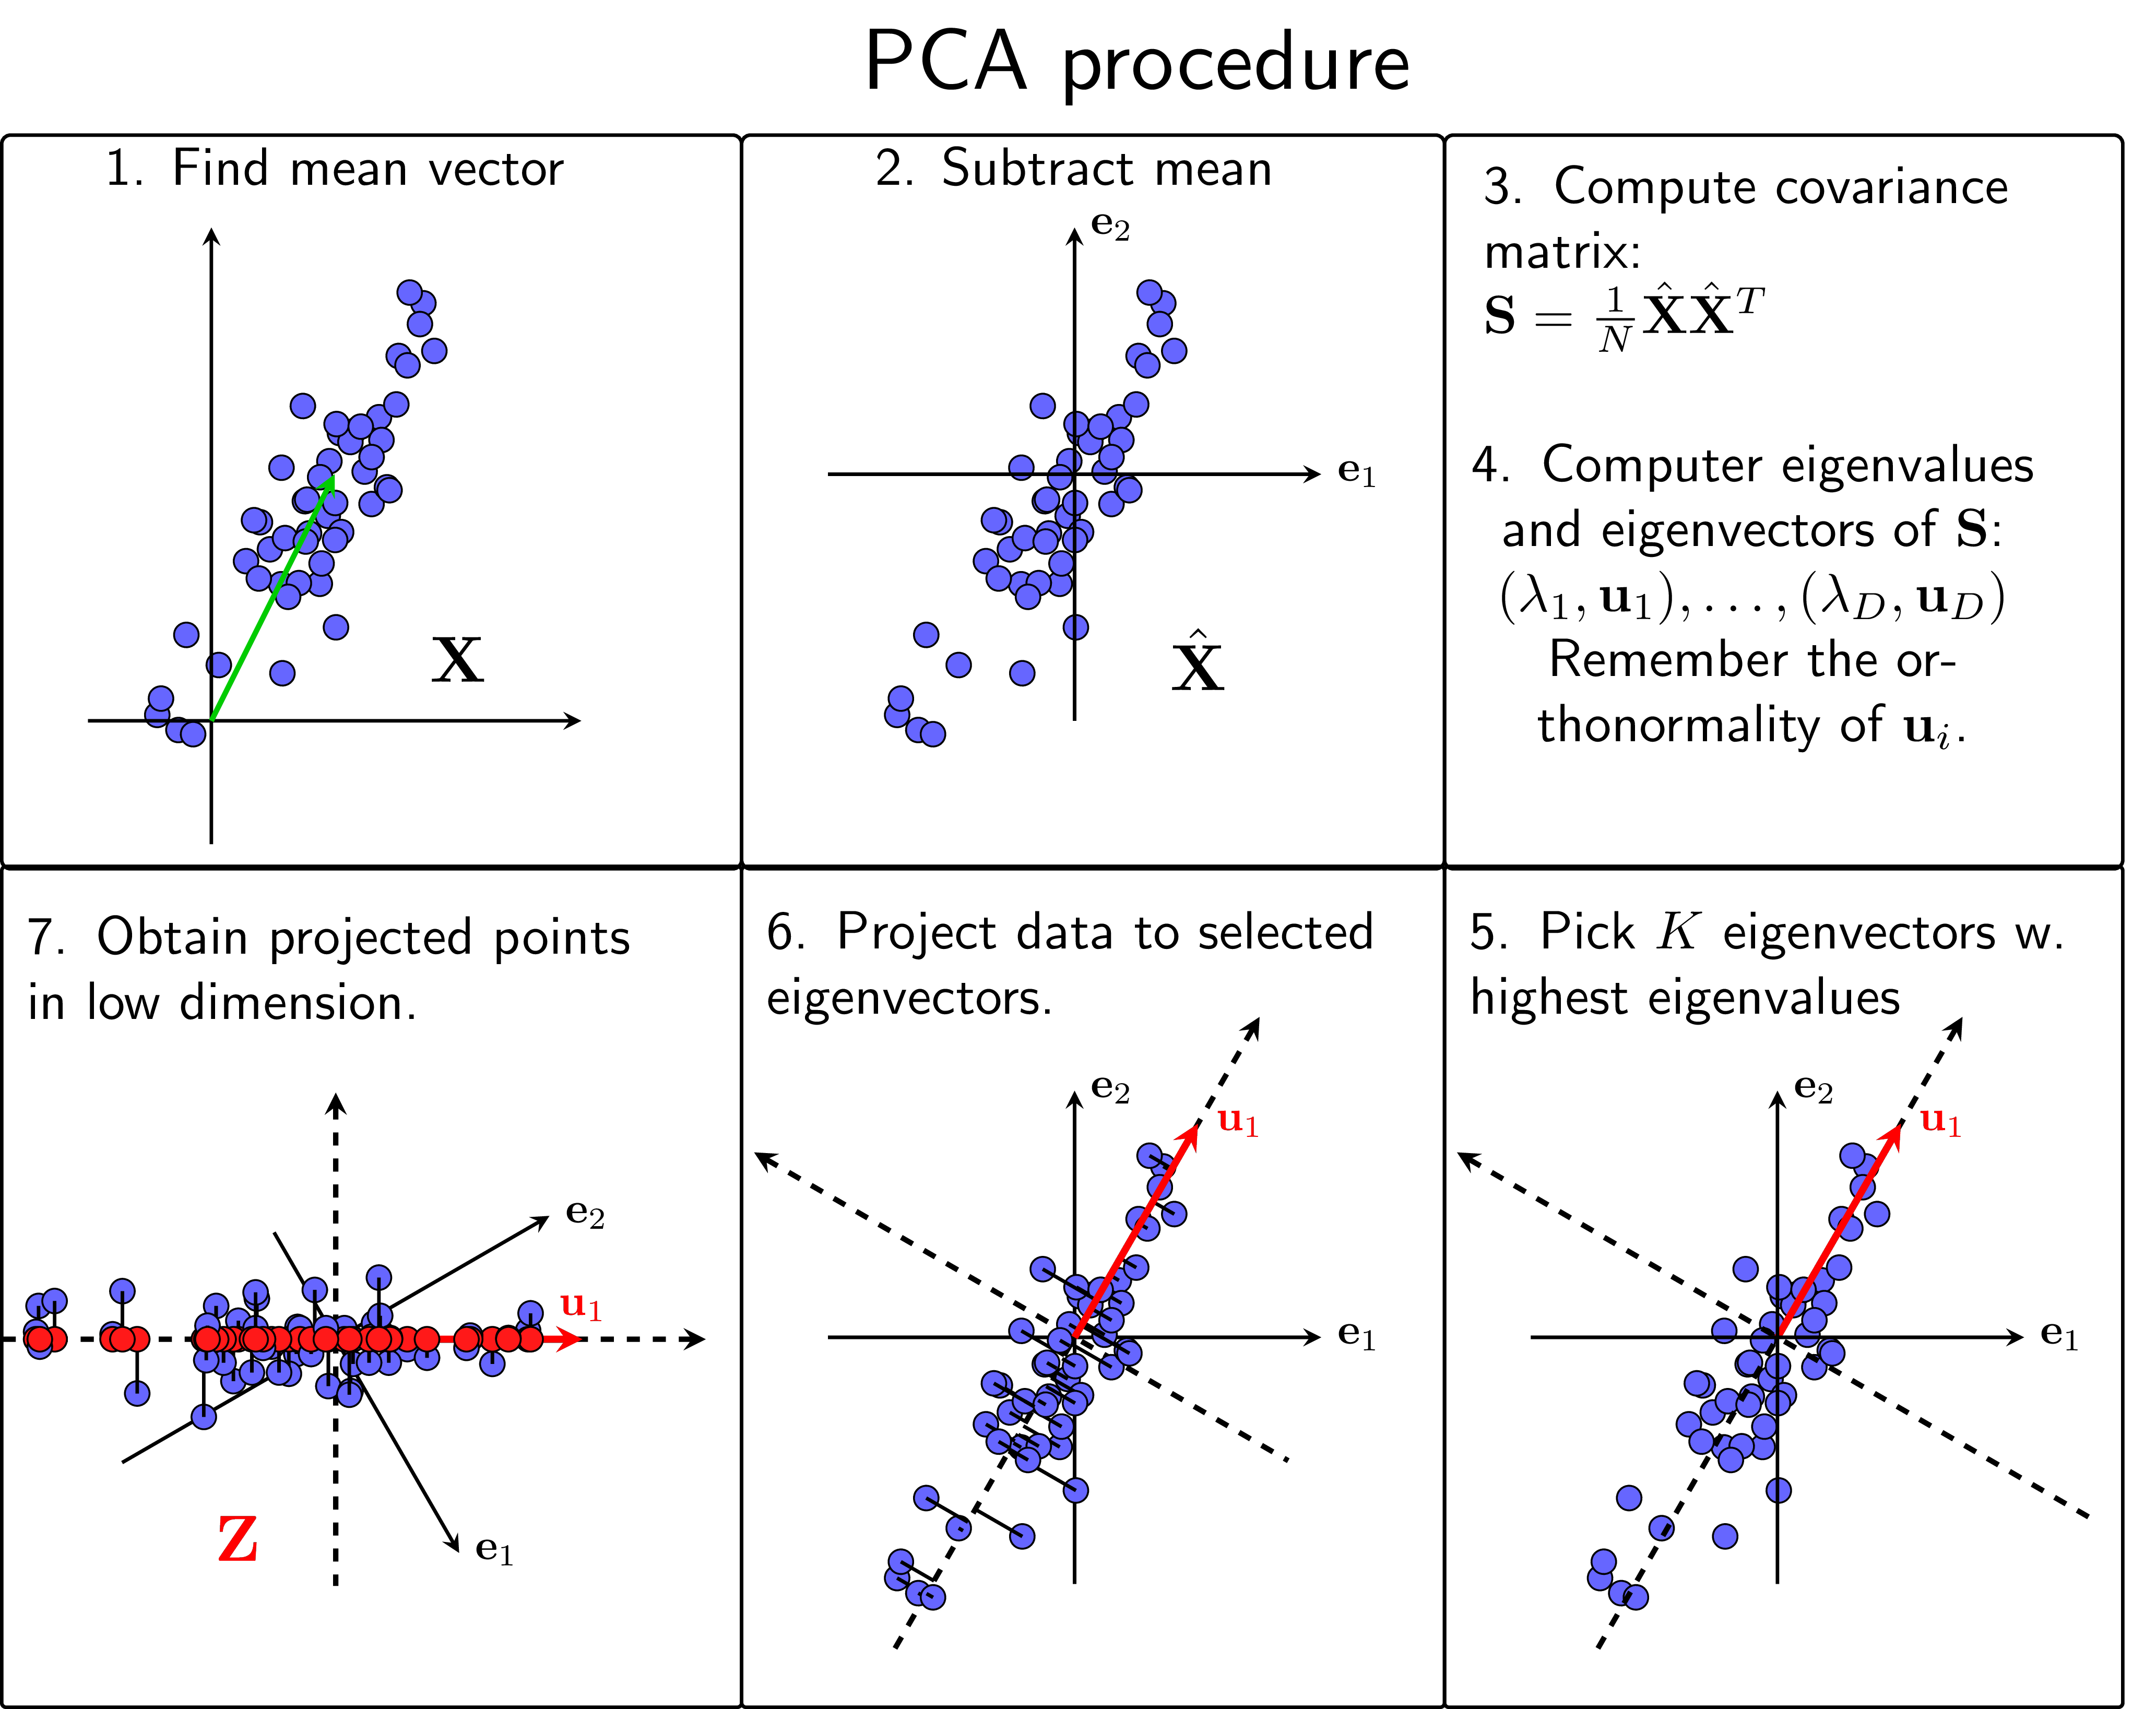
\includegraphics[scale=0.06]{pca_procedure.png}
    	\caption{PCA procedure, source: machinelearningcoban.com}
    \end{figure}
}

\frame{
\frametitle{Applications}
    \centering
    \begin{figure}
    	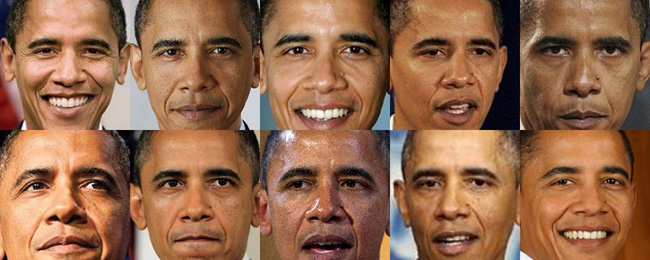
\includegraphics[scale=0.5]{obama.png}\\
    	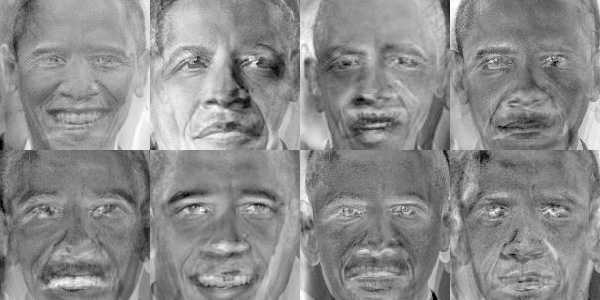
\includegraphics[scale=0.5]{eigenfaces.png}
    	\caption{Eigenfaces in face recognition.}
    \end{figure}
}

\frame{
\frametitle{t-Distributed Stochastic Neighbor Embedding (t-SNE)}
\centering
    \begin{figure}
    	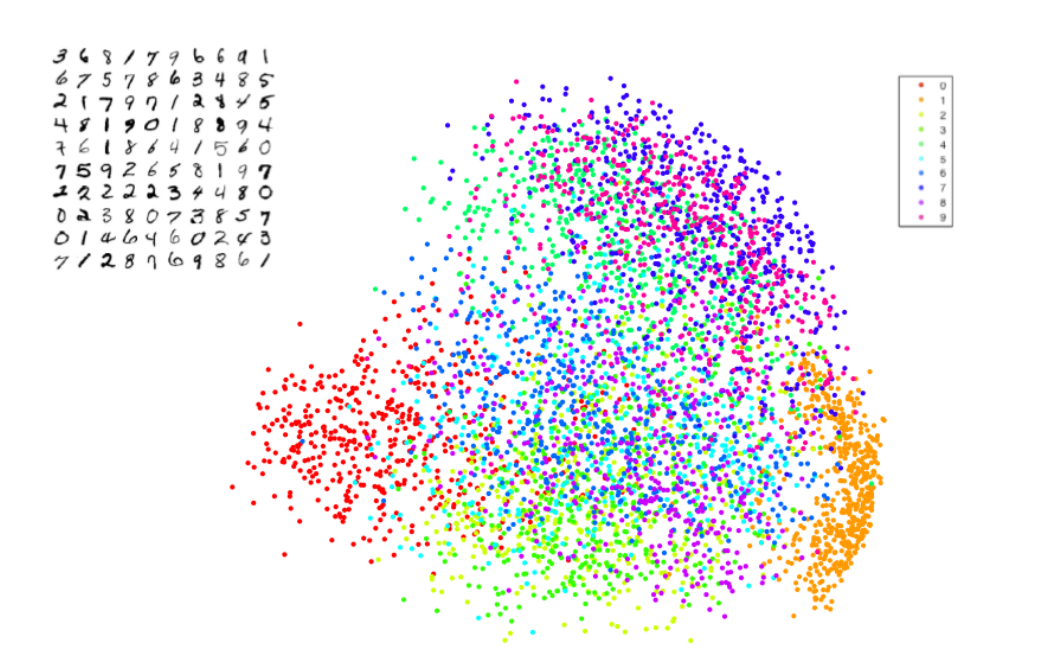
\includegraphics[scale=0.25]{pca-mnist-color.png}
    	\caption{PCA on MNIST dataset}
    \end{figure}
}

\frame{
\frametitle{t-Distributed Stochastic Neighbor Embedding (t-SNE)}
\centering
    \begin{figure}
    	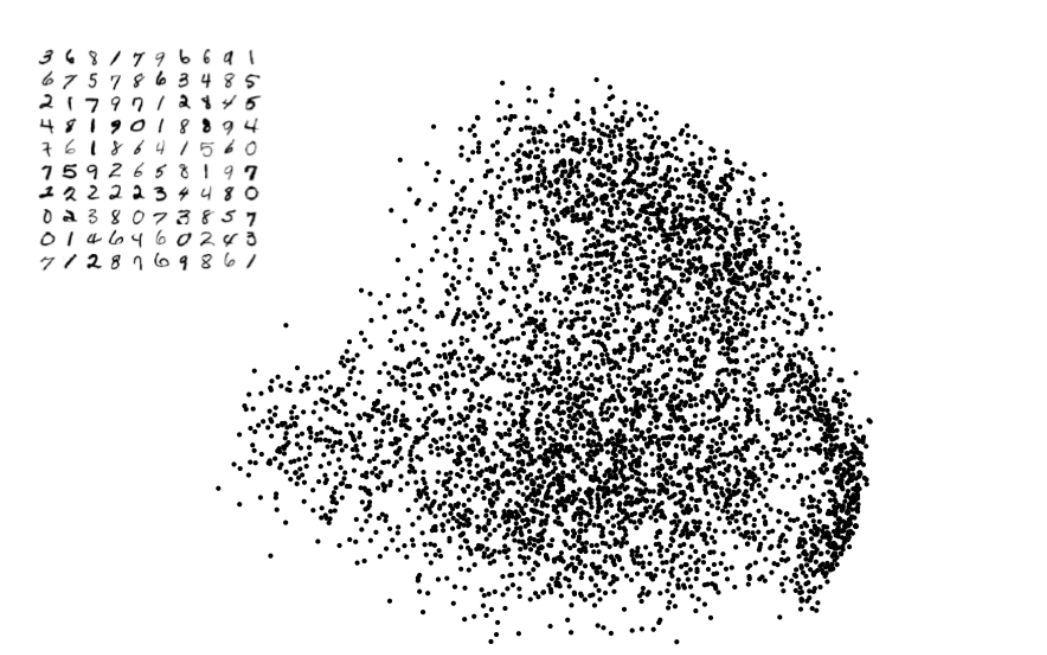
\includegraphics[scale=0.25]{pca-mnist-uncolor.png}
    	\caption{PCA on MNIST dataset}
    \end{figure}
}

\frame{
\frametitle{t-Distributed Stochastic Neighbor Embedding (t-SNE)}
\begin{itemize}
    \item How about non-linear data? 
\end{itemize}
\centering
    \begin{figure}
    	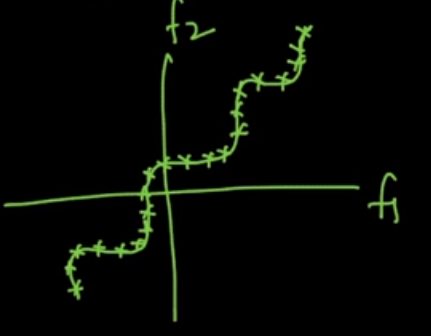
\includegraphics[scale=0.5]{nonlinear-dataset.png}
    \end{figure}
}

\frame{
\frametitle{t-Distributed Stochastic Neighbor Embedding (t-SNE)}
\begin{itemize}
    \item t-Distributed Stochastic Neighbor Embedding (t-SNE) is a non-linear technique for dimensionality reduction that is particularly well suited for the visualization of high-dimensional datasets.
    \item The t-SNE algorithm models the probability distribution of neighbors around each point, so it preserve the local structure (neigborhood) of data. 
\end{itemize}
}

\frame{
\frametitle{t-Distributed Stochastic Neighbor Embedding (t-SNE)}
\begin{itemize}
    \item Preserve the neighborhood 
\end{itemize}
\centering
    \begin{figure}
    	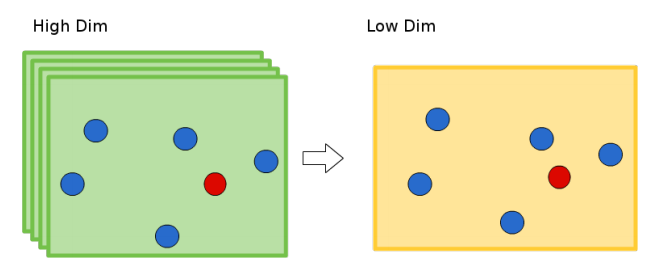
\includegraphics[scale=0.5]{tsne-highdimensional.png}
    \end{figure}
}

\frame{
\frametitle{t-Distributed Stochastic Neighbor Embedding (t-SNE)}
\begin{itemize}
    \item Converting the high-dimensional Euclidean distances into conditional
probabilities that represent similarities 
\end{itemize}
\centering
    \begin{figure}
    	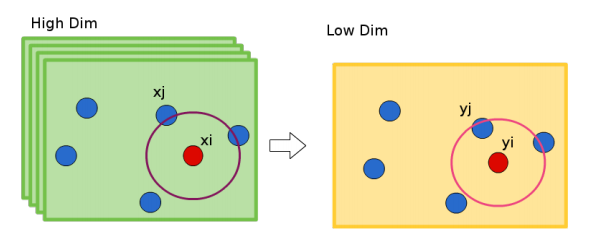
\includegraphics[scale=0.5]{tsne-gaussian.png}
    \end{figure}
 \begin{equation}
     p_{j|i} = \frac{\exp(-||x_i-x_j||^2/2\sigma^2)}{\sum_{j'\ne i}\exp(-||x_i-x_j'||^2/2\sigma^2)}
 \end{equation}
}


\frame{
\frametitle{t-Distributed Stochastic Neighbor Embedding (t-SNE)}
\begin{itemize}
    \item Converting the high-dimensional Euclidean distances into conditional
probabilities that represent similarities.
    \begin{equation}
     p_{j|i} = \frac{\exp(-||x_i-x_j||^2/2\sigma_i^2)}{\sum_{j'\ne i}\exp(-||x_i-x_j'||^2/2\sigma_i^2)}
    \end{equation}
    \item Since each point has different density, we'd use the symmetrized conditional:
    \begin{equation}
     p_{ij} = \frac{p_{j|i} + p_{i|j}}{2N}
    \end{equation}
    \item We set the bandwidth $\sigma_i$ such that the conditional has fixed \textit{perplexity}.
    \begin{equation}
     Perp(P_i) = 2^{-\sum_{j}p_{j|i}log_2p_j}
    \end{equation}
\end{itemize}
}

\frame{
\frametitle{t-Distributed Stochastic Neighbor Embedding (t-SNE)}
\begin{itemize}
    \item Similarity in low dimension is measured as:
    \begin{equation}
     q_{ij} = \frac{(1+||y_i-y_j||^2)^-1}{\sum_{k} \sum_{l\ne k}(1+||y_k-y_l||^2)^-1}
    \end{equation}
\end{itemize}
}

\frame{
\frametitle{t-Distributed Stochastic Neighbor Embedding (t-SNE)}
\begin{itemize}
    \item Cost function: Kullback Leibler (KL) divergence:
    \begin{equation}
     KL(P||Q) = \sum_i \sum_{j \ne i} p_{ij} log \frac{p_{ij}}{q_{ij}}
    \end{equation}
    \begin{itemize}
        \item Large $p_{ij}$ modeled by small $q_{ij}$: $\rightarrow$ Big penalty.
        \item Small $p_{ij}$ modeled by large $q_{ij}$: $\rightarrow$ Small penalty.
        \item t-SNE mainly preserves local similarity structure of data. 
    \end{itemize}
    \item Gradient:
    \begin{equation}
        \frac{\partial C}{\partial y_i} = 4 \sum_{j \ne i} (p_{ij} - q_{ij})(1+||y_i-y_j||^2)^-1(y_i-y_j)
    \end{equation}
    
\end{itemize}
}

\frame{
\frametitle{t-Distributed Stochastic Neighbor Embedding (t-SNE)}
\centering
    \begin{figure}
    	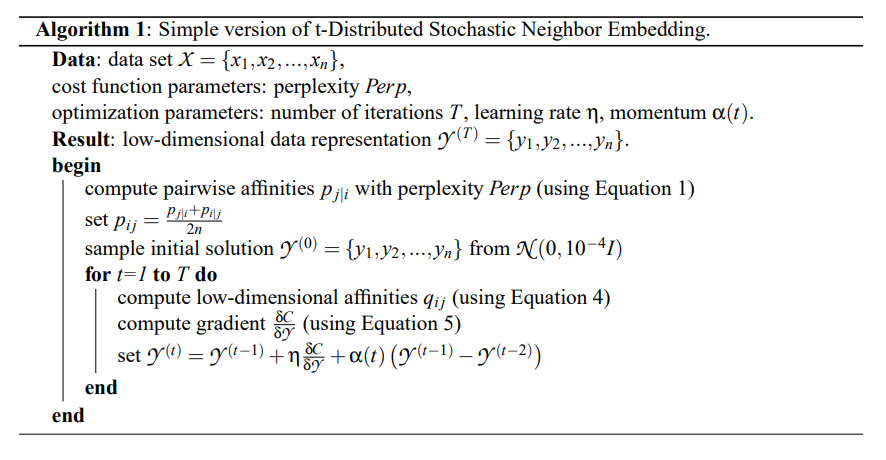
\includegraphics[scale=0.5]{tsne-algorithm.png}
    	\caption{t-SNE learning algorithm}
    \end{figure}
}

\frame{
\frametitle{t-Distributed Stochastic Neighbor Embedding (t-SNE)}
\centering
    \begin{figure}
    	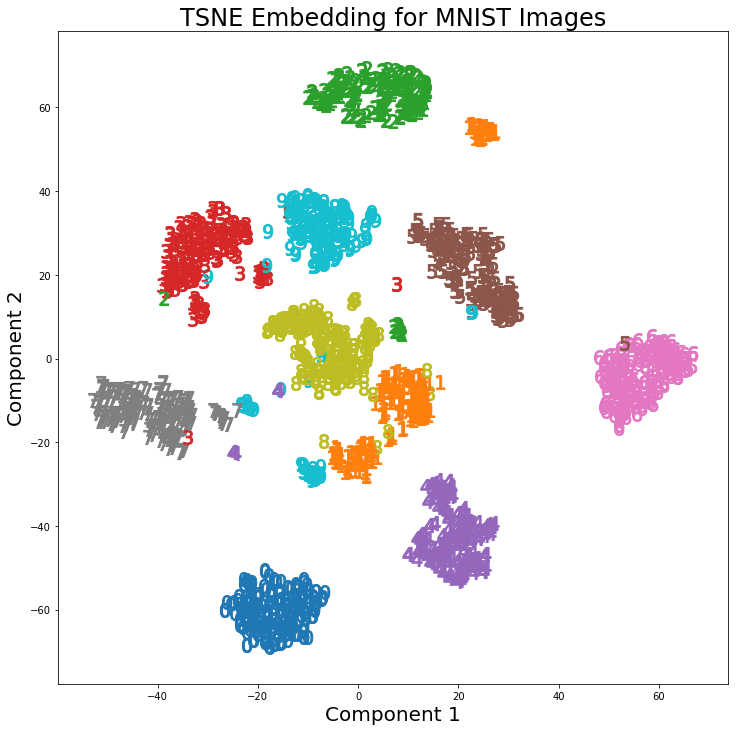
\includegraphics[scale=0.35]{tsne-mnist.png}
    	\caption{t-SNE on MNIST dataset}
    \end{figure}
}

\frame{
\frametitle{PCA vs t-SNE}
\begin{itemize}
    \item t-SNE is computationally expensive and can take several hours on million-sample datasets where PCA will finish in seconds or minutes.
    \item Linear dimensionality reduction algorithms, like PCA, concentrate on placing dissimilar data points far apart in a lower dimension.
    \item But in order to represent high dimension data on low  dimension, non-linear manifold, it is essential that similar data points must be represented close together, which is something t-SNE does, not PCA.
    \item Since PCA is a linear algorithm, it will not be able to interpret the complex polynomial relationship between features while t-SNE is made to capture exactly that representation.
    \item Since t-SNE is parameterless, everytime new data comes in, t-SNE has to learn new embedding for that data. While PCA can be used a feature extraction function (eigenface for example).
    
\end{itemize}
}


\frame{
\frametitle{References}
[1] Richard Johnson et al, Applied Multivariate Statistical Analysis 6th Edition.

[2] Tiep H. Vu, Principal Component Analysis, https://machinelearningcoban.com/2017/06/15/pca/

[3] Laurens van der Maaten \& Geoffrey Hinton, Visualizing Data using t-SNE.

[4] Manifold learning, https://scikit-learn.org/stable/modules/manifold.html.
}
\end{document}
